% \newpage
\chapter{IMPLEMENTATION}
\pagestyle{fancy}
% \begin{center}
% % \textbf{\LARGE \centering IMPLEMENTATION}\\[1cm]
% \end{center}
\justify
\begin{figure}[h]  % 'h' means place here
    \centering
    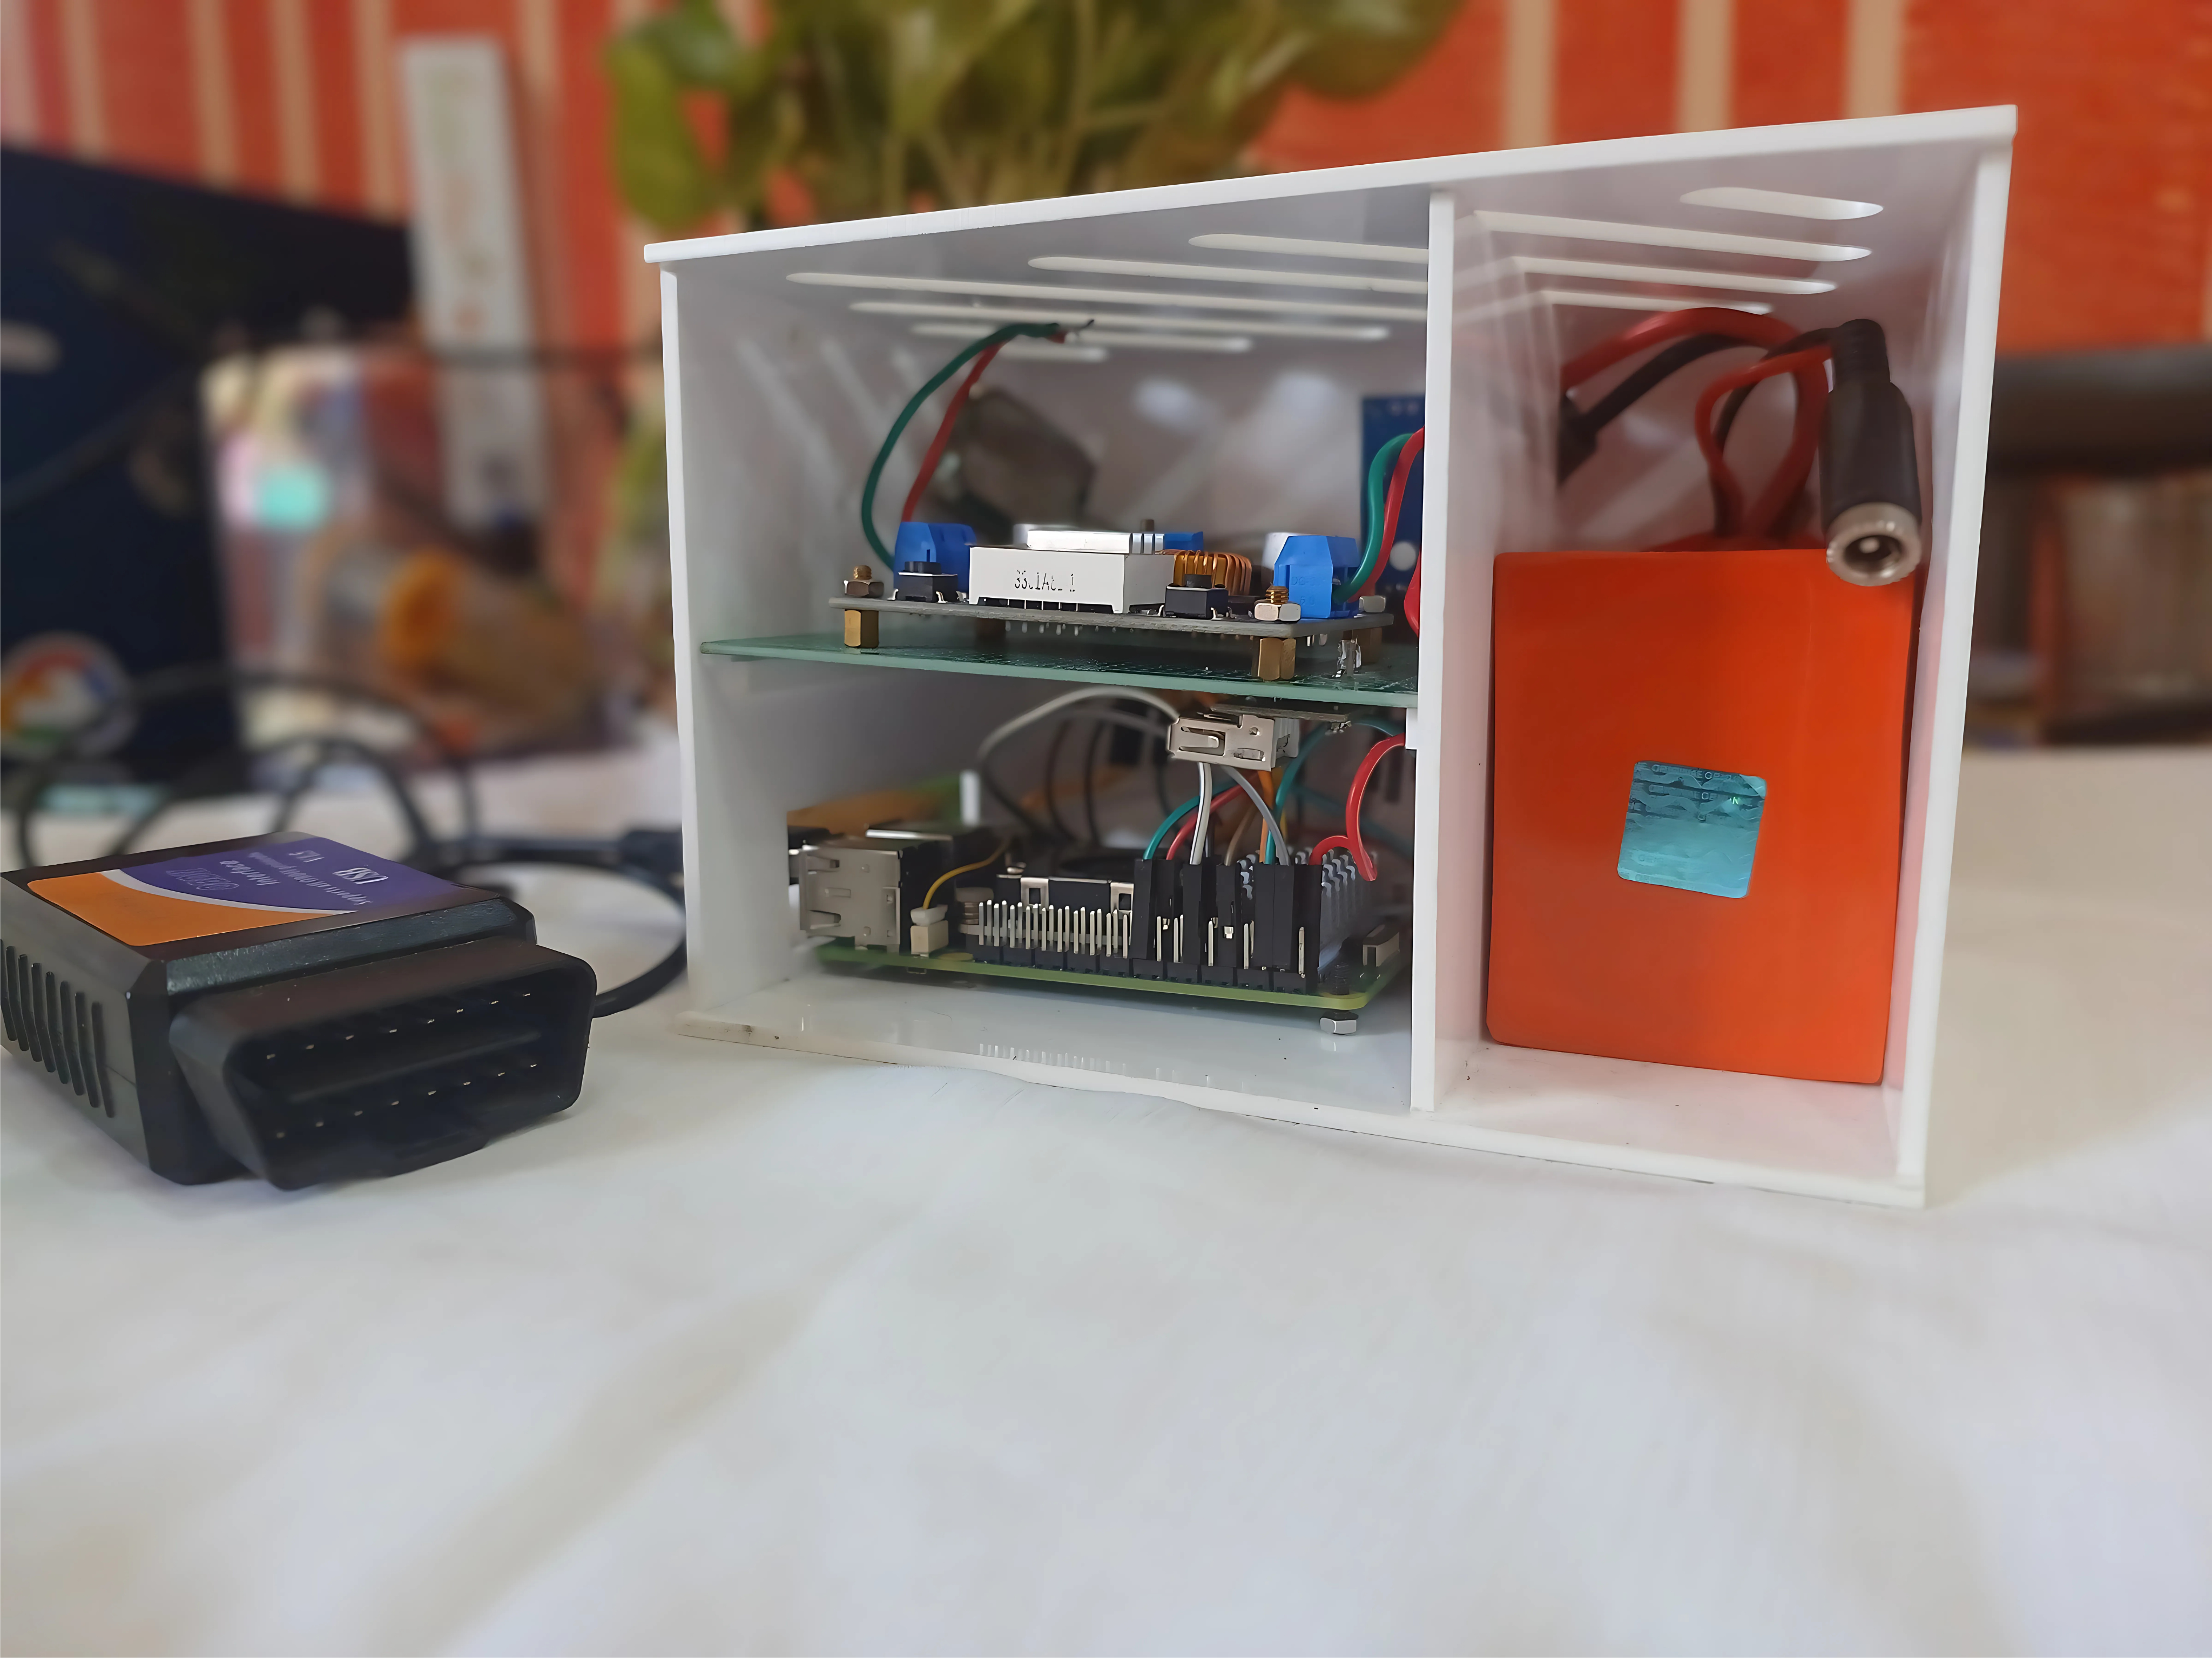
\includegraphics[width=0.75\textwidth]{assets/Untitleddesign.png}
    \caption{Automotive Diagnostic And Activity Monitoring (ADAM) BOX}
    \label{fig:ADAM Box}
\end{figure}
\section{INTRODUCTION}

This chapter discusses the implementation of our system, which consists of three primary components: the hardware setup, cloud-based storage and analysis, and a mobile application for user interaction.
    \subsection{HARDWARE IMPLEMENTATION}
        The hardware implementation consists of multiple sensors connected to a Raspberry Pi 5, serving as the central edge computing unit for real-time data acquisition, local processing, and cloud transmission. The system integrates several key components:
        \begin{itemize}
            \item Raspberry Pi 5: Acts as the central processing unit, efficiently handling real-time data acquisition, local computation, and sensor coordination
            \item GPS Module (NEO-6M): Enables accurate vehicle location tracking and route history monitoring
            \item Vibration Sensor (SW-420): Detects collision events and unusual vibrations indicative of accidents or aggressive driving patterns
            \item Gyroscope Module: Monitors vehicle orientation, tilt, and angular motion for advanced motion analysis, including rollover detection and abrupt turn identification
            \item Power Management: Connected to the vehicle battery via a relay system to prevent direct current cut-off when the car is turned off, ensuring continuous monitoring capability
        \end{itemize}
        \begin{figure}[h]
            \centering
            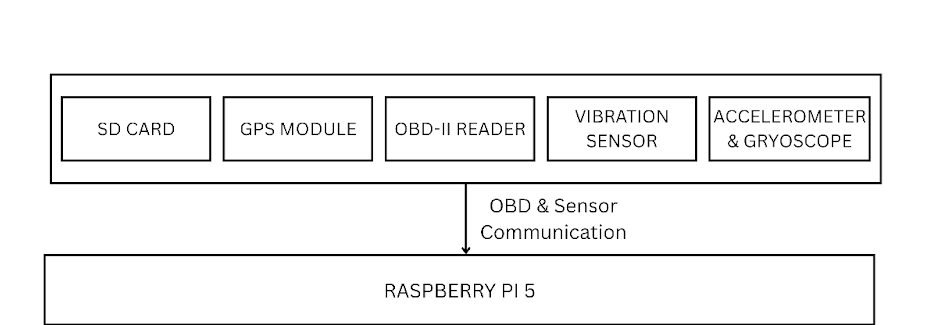
\includegraphics[width=1\textwidth]{assets/flow_diagram_hardware.png}
            \caption{Flow Diagram Of Raspberry pi}
            \label{fig:Flow Diagram}
        \end{figure}
        \begin{lstlisting}[
            language=Python,
            caption={Main Hardware Implementation Function},
            label={lst:hardware_main},
            basicstyle=\small\ttfamily,
            frame=tb,
            framerule=0.5pt,
            breaklines=true,
            showstringspaces=false,
            numbers=left,
            stepnumber=1,
            tabsize=4,
            captionpos=t,
            xleftmargin=0.5cm,
            xrightmargin=0.5cm,
            aboveskip=1em,
            belowskip=1em
        ]
def main():
    """
    Main hardware implementation function for edge-based automotive data collection
    Demonstrates parallel sensor data acquisition, local preprocessing, and cloud transmission
    """
    global Async_conn, esp_conn, running
    
    print("Initializing ADAM - Automotive Data Acquisition Module")
    
    # Read configuration parameters
    obd_port, esp8266_port, esp8266_baud, sensor_file, temp_csv_path, data_csv_path, server_url = read_config()
    
    try:
        # Initialize hardware connections
        Async_conn = Async_connection(obd_port)  # OBD-II interface
        esp_conn = Esp8266_conn(esp8266_port, esp8266_baud)  # ESP8266 sensor module
        
        print(f"Hardware initialized - OBD: {obd_port} | ESP8266: {esp8266_port}")
        
        # Main data collection loop
        iteration = 1
        while running:
            print(f"\n--- Data Collection Cycle {iteration} ---")
            
            # Parallel sensor data acquisition
            results = {}
            
            # Create concurrent threads for multi-sensor data collection
            obd_thread = threading.Thread(
                target=collect_obd_data, 
                args=(Async_conn, 1, sensor_file, results)
            )
            esp_thread = threading.Thread(
                target=collect_serial_data,
                args=(esp_conn, results)
            )
            
            # Execute parallel data collection
            obd_thread.start()
            esp_thread.start()
            obd_thread.join()
            esp_thread.join()
            
            # Local preprocessing and data fusion
            if 'obd_df' in results and 'serial_df' in results:
                combined_df = merge_dataframes(results['obd_df'], results['serial_df'])
                
                # Edge processing: Save locally with timestamp
                combined_df.to_csv(temp_csv_path, index=False)
                append_to_data_csv(temp_csv_path, data_csv_path)
                
                # Cloud transmission for centralized analysis
                upload_result = upload_to_server(temp_csv_path, server_url)
                
                print(f"Cycle {iteration} complete - Data processed and transmitted")
            
            iteration += 1
            time.sleep(1)  # Regular interval collection
            
    except Exception as e:
        print(f"Hardware implementation error: {e}")
    finally:
        # Cleanup hardware connections
        if Async_conn: Async_conn.close()
        if esp_conn: esp_conn.close()

def merge_dataframes(obd_df, serial_df):
    """
    Local preprocessing: Merge multi-sensor data with timestamp synchronization
    """
    obd_df = obd_df.reset_index(drop=True)
    serial_df = serial_df.reset_index(drop=True)
    
    # Add synchronized timestamp for data correlation
    timestamp = datetime.now().strftime("%Y-%m-%d %H:%M:%S")
    obd_df["MERGED_TIMESTAMP"] = timestamp
    
    # Horizontal concatenation for unified sensor data
    combined_df = pd.concat([obd_df, serial_df], axis=1)
    return combined_df

        \end{lstlisting}

        The Raspberry Pi collected sensor data at regular intervals, pre-processed it locally, and transmitted the information to a cloud backend for storage and analysis. This edge setup ensured low-latency data capture and immediate response to critical driving events.

\section{GOLANG}
    Once data is collected and processed locally by the Raspberry Pi 5 edge device, it is transmitted to a Golang-based server which acts as a middleware communication layer. This Go server ensures the reliable and secure transmission of structured telemetry data from edge to backend systems, enabling near real-time monitoring and decision-making.
    The Go server exposes a set of RESTful API endpoints for interacting with various components of the data pipeline. These include:
    \begin{enumerate}
        \item \textbf{/upload:} 
            Handles incoming CSV files via POST requests. Data is parsed using Go’s CSV reader libraries, and SQL queries are dynamically constructed for storage in the PostgreSQL database.
            \begin{lstlisting}[
                language=Go, 
                caption={Upload CSV Route Handler},
                basicstyle=\small\ttfamily,
                frame=tb,
                framerule=0.5pt,
                breaklines=true,
                showstringspaces=false,
                numbers=left,
                stepnumber=1,
                tabsize=4,
                captionpos=t,
                xleftmargin=0.5cm,
                xrightmargin=0.5cm,
                aboveskip=1em,
                belowskip=1em
            ]
func UploadHandler(c *fiber.Ctx) error {
    file, _ := c.FormFile("file")
    f, _ := file.Open()
    defer f.Close()

    r := csv.NewReader(f)
    header, _ := r.Read()
    records, _ := r.ReadAll()

    table := "telemetry"
    cols := strings.Join(header, " TEXT, ") + " TEXT"
    query := fmt.Sprintf(
        "CREATE TABLE IF NOT EXISTS %s (%s);",
        table, cols)

    conn, _ := database.GetPool().
        Acquire(context.Background())
    defer conn.Release()
    conn.Exec(context.Background(), query)

    placeholders := make([]string, len(header))
    for i := range header {
        placeholders[i] = fmt.Sprintf("$%d", i+1)
    }

    insert := fmt.Sprintf(
        "INSERT INTO %s (%s) VALUES (%s)",
        table,
        strings.Join(header, ", "),
        strings.Join(placeholders, ", "),
    )

    for _, rec := range records {
        conn.Exec(
            context.Background(),
            insert,
            toIfaceSlice(rec)...,
        )
    }
    return c.SendStatus(200)
}
            \end{lstlisting}
        \item \textbf{/data:} 
            Allows GET requests to fetch the most recent or specific historical records from the database. This enables dashboards, apps, or other services to retrieve and display relevant vehicle data.
            \begin{lstlisting}[
                language=Go, 
                caption={Data Retrieval Route Handler},
                basicstyle=\small\ttfamily,
                frame=tb,
                framerule=0.5pt,
                breaklines=true,
                showstringspaces=false,
                numbers=left,
                stepnumber=1,
                tabsize=4,
                captionpos=t,
                xleftmargin=0.5cm,
                xrightmargin=0.5cm,
                aboveskip=1em,
                belowskip=1em
            ]
func FetchHandler(c *fiber.Ctx) error {
    pool := database.GetPool()
    conn, err := pool.Acquire(context.Background())
    if err != nil {
        log.Printf("DB connection error: %v", err)
        return c.Status(500).JSON(
            fiber.Map{"error": "DB error"})
    }
    defer conn.Release()

    table := "dataset"
    query := `SELECT * FROM ` + table
    rows, err := conn.Query(context.Background(), query)
    if err != nil {
        log.Printf("Query error: %v", err)
        return c.Status(500).JSON(
            fiber.Map{"error": "Query error"})
    }
    defer rows.Close()

    fields := rows.FieldDescriptions()
    columns := make([]string, len(fields))
    for i, f := range fields {
        columns[i] = string(f.Name)
    }

    var result []map[string]interface{}
    for rows.Next() {
        row := make([]interface{}, len(columns))
        ptrs := make([]interface{}, len(columns))
        for i := range row {
            ptrs[i] = &row[i]
        }
        if err := rows.Scan(ptrs...); err != nil {
            log.Printf("Scan error: %v", err)
            return c.Status(500).JSON(
                fiber.Map{"error": "Scan error"})
        }
        rowMap := make(map[string]interface{})
        for i, col := range columns {
            if v, ok := row[i].([]uint8); ok {
                rowMap[col] = string(v)
            } else {
                rowMap[col] = row[i]
            }
        }
        result = append(result, rowMap)
    }

    if err := rows.Err(); err != nil {
        log.Printf("Row iteration error: %v", err)
        return c.Status(500).JSON(
            fiber.Map{"error": "Read error"})
    }

    return c.JSON(fiber.Map{
        "data":    result,
        "count":   len(result),
        "columns": columns,
    })
}
            \end{lstlisting}
        \item \textbf{/health:} 
            A lightweight endpoint that returns the server's health status, used for monitoring and diagnostics.
            \begin{lstlisting}[
                language=Go, 
                caption={Health Check Route Handler},
                basicstyle=\small\ttfamily,
                frame=tb,
                framerule=0.5pt,
                breaklines=true,
                showstringspaces=false,
                numbers=left,
                stepnumber=1,
                tabsize=4,
                captionpos=t,
                xleftmargin=0.5cm,
                xrightmargin=0.5cm,
                aboveskip=1em,
                belowskip=1em
            ]
var startTime = time.Now()

func HealthHandler(c *fiber.Ctx) error {
    healthData := map[string]interface{}{
        "status":    "healthy",
        "uptime":    utils.GetUptime(startTime),
        "timestamp": time.Now().
            Format(time.RFC3339),
    }

    return c.Status(fiber.StatusOK).
        JSON(healthData)
}

            \end{lstlisting}
    \end{enumerate}
    Through these endpoints, the Go server functions as the key intermediary for reliable, flexible, and secure data ingestion into the centralized storage system.
\section{POSTGRES DB}
    The collected data is stored in a PostgreSQL (PGSQL) database for future processing and analysis. This database serves as the central repository for storing vehicle data, including various parameters like engine temperature, fuel consumption, speed, and more. The structured format of the database allows for efficient querying and data retrieval.
    All incoming telemetry and diagnostic data are stored in a PostgreSQL (PGSQL) relational database, which acts as the core data repository for the ADAM system. PostgreSQL is selected due to its enterprise-level capabilities, including full support for ACID transactions, advanced indexing techniques, query optimization, and secure storage features.
    The PostgreSQL database is designed with a normalized schema that efficiently captures and organizes various datasets such as:
    Engine diagnostic parameters and fault codes

    \begin{itemize}
        \item GPS and route tracking logs
        \item Vehicle movement and sensor activity
        \item Temperature metrics and thermal events
        \item User metadata and access logs
    \end{itemize}
    Structured storage facilitates rapid query response times and easy retrieval of records for downstream analytics and machine learning tasks. This centralized repository ensures long-term archival, auditability, and scalability as data volume grows.

\section{FASTAPI}
    Once stored, the diagnostic data is accessed by a FastAPI-based application layer. This server plays a central role in processing data, serving APIs to external interfaces, and executing real-time and scheduled analysis tasks. One of its most critical roles is the application of Machine Learning (ML) models trained on historical vehicle data to derive predictive insights.
    \begin{enumerate}
        \item \textbf{Emissions Diagnostic:} 
            The emissions router (\path{routers/emissions.py}) processes real-time sensor data to determine emission compliance status using the EnhancedCarEmissionsMLModel. When a request is received, the router accepts CSV uploads or JSON payloads containing sensor readings such as CO levels, NOx concentrations, and particulate matter measurements. The data is validated using Pydantic models before being passed to the emissions model, which preprocesses the sensor values, applies Indian emission standard thresholds, and generates compliance classifications using a trained Random Forest classifier. The router returns structured JSON responses containing compliance status, confidence scores, and detailed sensor analysis, along with optional confusion matrix visualizations for model performance assessment.
        \item \textbf{Engine Health Diagnostic:} 
            As part of the \textbf{ADAM system}, an engine health monitoring module was built using a \textbf{Random Forest Classifier} trained on OBD-II vehicle telemetry. The model classifies engine condition as \textit{"Good"} or \textit{"Needs Attention"}, enabling predictive maintenance and improving vehicle safety.

            \subsection*{Workflow}

            \begin{itemize}
                \item OBD-II data (RPM, throttle position, temperature, voltage, misfire counts, etc.) is preprocessed and labeled as healthy or faulty.
                \item Data split: \textbf{70\% training}, \textbf{30\% testing}.
                \item The Random Forest model is trained and tested, achieving \textbf{92\% accuracy}, with perfect precision and recall.
                \item Feature importance analysis identified RPM, coolant temperature, throttle position, misfire counts, and control module voltage as key predictors.
            \end{itemize}
            \begin{table}[H]
                \centering
                \caption{Internal Evaluation on Expert Data (Engine Health Classification)}
                \label{tab:engine_health_evaluation}
                \begin{tabular}{|l|c|c|c|c|}
                    \hline
                    \textbf{Class} & \textbf{Precision} & \textbf{Recall} & \textbf{F1-Score} & \textbf{Support} \\
                    \hline
                    \texttt{bb} (Needs Attention) & 0.85 & 0.85 & 0.85 & 48 \\
                    \texttt{gg} (Good)             & 0.95 & 0.95 & 0.95 & 137 \\
                    \hline
                    \textbf{Accuracy}              & \multicolumn{4}{|c|}{0.92 (185 samples)} \\
                    \hline
                    \textbf{Macro Average}         & 0.90 & 0.90 & 0.90 & 185 \\
                    \hline
                    \textbf{Weighted Average}      & 0.92 & 0.92 & 0.92 & 185 \\
                    \hline
                \end{tabular}
            \end{table}

            \subsection*{Router Function}

            The \path{engine_health.py} router processes incoming OBD data, runs it through the trained model, and returns a health status report with:
            \begin{itemize}
                \item Predicted engine condition
                \item Anomaly detection insights
                \item Maintenance recommendations
            \end{itemize}

            A distribution graph visualizes occurrences of predicted engine conditions across the dataset, as shown in \textbf{Figure~\ref{fig:engine_condition_distribution}}.

            \begin{figure}[H]
                \centering
                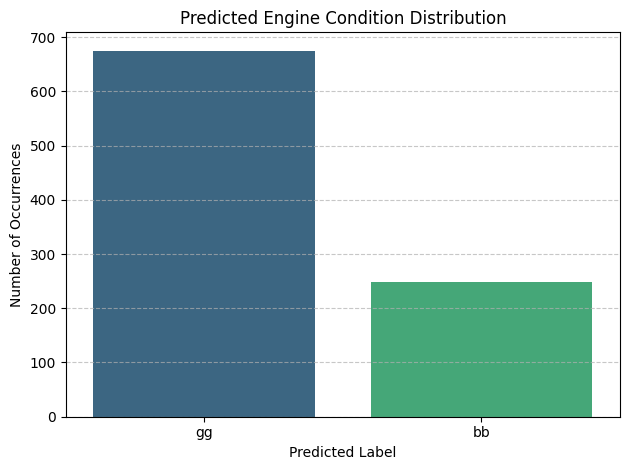
\includegraphics[width=0.7\textwidth]{assets/predeicte image.png}
                \caption{Predicted Engine Condition Distribution (Good vs. Needs Attention)}
                \label{fig:engine_condition_distribution}
            \end{figure}

        \item \textbf{Predictive Maintenance System:} 
        The \textbf{Predictive Maintenance Router} (\path{routers/predictive\_maintenance.py}) serves as a cornerstone module within the \textbf{ADAM system}, engineered to deliver comprehensive fleet maintenance analytics through automated diagnostic workflows. The system integrates real-time vehicle telemetry processing with rule-based maintenance scheduling to ensure optimal fleet operational reliability.

        \subsection{System Architecture and Data Processing}
        
        The predictive maintenance module employs a multi-stage processing pipeline that transforms raw sensor data into actionable maintenance insights. The core implementation leverages the \texttt{VehicleMaintenance} class to systematically evaluate vehicle health metrics including mileage progression, engine operational parameters, sensor performance indicators, and historical usage patterns.

        \begin{lstlisting}[
            language=Python,
            caption={Main Hardware Implementation Function},
            label={lst:hardware_main},
            basicstyle=\small\ttfamily,
            frame=tb,
            framerule=0.5pt,
            breaklines=true,
            showstringspaces=false,
            numbers=left,
            stepnumber=1,
            tabsize=4,
            captionpos=t,
            xleftmargin=0.5cm,
            xrightmargin=0.5cm,
            aboveskip=1em,
            belowskip=1em
            ]
@router.get("/diagnose")
def generate_predictive_diagnosis():
    """
    Comprehensive endpoint that runs all maintenance diagnostics and generates a detailed report.
    """
    global maintenance_reports, predictive_report

    try:
        # Step 1: Fetch Data
        print("\n[1/4] Fetching maintenance data...")
        conn = connect_to_db()
        query = "SELECT * FROM kaiserskoda;"
        df = pd.read_sql(query, conn)
        conn.close()
        print(" Data fetched successfully")

        # Step 2: Preprocess
        print("\n[2/4] Preprocessing maintenance data...")
        processed_df = preprocess_data(df)
        print(" Preprocessing complete")

        # Step 3: Generate Vehicle Reports
        print("\n[3/4] Analyzing vehicle conditions...")
        reports = []
        maintenance_statuses = {
            'Critical': 0,
            'Warning': 0,
            'Good': 0
        }

        for idx, row in processed_df.iterrows():
            try:
                vehicle = VehicleMaintenance(
                    distance_w_mil=row["distance_w_mil"],
                    time_in_years=row["time_in_years"],
                    speed=row["speed"],
                    engine_load=row["engine_load"],
                    coolant_temp=row["coolant_temp"],
                    run_time=row["run_time"],
                    throttle_pos=row["throttle_pos"],
                    control_module_voltage=row["control_module_voltage"],
                    fuel_level=row["fuel_level"],
                    short_fuel_trim_1=row["short_fuel_trim_1"],
                    long_fuel_trim_1=row["long_fuel_trim_1"],
                    ambiant_air_temp=row["ambiant_air_temp"],
                    o2_sensors=row["o2_sensors"],
                    catalyst_temp_b1s1=row["catalyst_temp_b1s1"]
                )

                report = vehicle.generate_report()

                # Determine vehicle status based on conditions
                critical_conditions = [
                    "immediately" in str(status).lower()
                    for status in report.values()
                    if isinstance(status, str)
                ]
                warning_conditions = [
                    "soon" in str(status).lower()
                    for status in report.values()
                    if isinstance(status, str)
                ]

                if any(critical_conditions):
                    report['overall_status'] = 'Critical'
                    maintenance_statuses['Critical'] += 1
                elif any(warning_conditions):
                    report['overall_status'] = 'Warning'
                    maintenance_statuses['Warning'] += 1
                else:
                    report['overall_status'] = 'Good'
                    maintenance_statuses['Good'] += 1

                reports.append(report)

            except Exception as e:
                logging.error(f"Error processing vehicle {idx}: {str(e)}")
                continue

        if not reports:
            raise ValueError("No valid reports were generated")

        maintenance_reports = pd.DataFrame(reports)

        # Step 4: Generate Summary Report
        print("\n[4/4] Generating comprehensive maintenance report...")

        summary_stats = {
            "timestamp": "2025-01-19 09:21:26",
            "total_vehicles": len(reports),
            "status_distribution": maintenance_statuses,
            "critical_systems": {
                "engine": maintenance_reports['Engine Load'].mean() if 'Engine Load' in maintenance_reports else 0,
                "coolant": maintenance_reports[
                    'Coolant Temperature'].mean() if 'Coolant Temperature' in maintenance_reports else 0,
                "fuel": maintenance_reports['Fuel Level'].mean() if 'Fuel Level' in maintenance_reports else 0,
                "brake_wear": maintenance_reports[
                    'Brake Pad Wear'].mean() if 'Brake Pad Wear' in maintenance_reports else 0
            },
            "maintenance_required": {
                "immediate_attention": maintenance_statuses['Critical'],
                "soon_attention": maintenance_statuses['Warning'],
                "good_condition": maintenance_statuses['Good']
            }
        }

        # Store the full report
        predictive_report = maintenance_reports.copy()
        predictive_report['analysis_timestamp'] = "2025-01-19 09:21:26"

        print("\nMaintenance Analysis Summary:")
        print(f"Total Vehicles Analyzed: {summary_stats['total_vehicles']}")
        print(f"Critical Issues: {maintenance_statuses['Critical']}")
        print(f"Warnings: {maintenance_statuses['Warning']}")
        print(f"Good Condition: {maintenance_statuses['Good']}")

        return {
            "summary": summary_stats,
            "report_preview": predictive_report.head(10).to_dict(orient="records"),
            "timestamp": "2025-01-19 09:21:26"
        }

    except Exception as e:
        logging.error(f"Error in predictive diagnosis: {str(e)}")
        raise HTTPException(
            status_code=500,
            detail=f"Error generating predictive maintenance report: {str(e)}"
        )
        \end{lstlisting}

        \subsection{Rule-Based Diagnostic Framework}
        
        Distinguished from machine learning approaches utilized in other system modules, the predictive maintenance router implements deterministic, threshold-based algorithms derived from OEM specifications and empirical operational data. This methodology ensures consistent, interpretable diagnostic outcomes across diverse vehicle configurations and operational environments.

        The diagnostic evaluation framework, as depicted in \textbf{Figure \ref{fig:predictive-maintenance-flowchart}}, processes real-time sensor data through the OBD-II interface and applies conditional assessment protocols across critical vehicle subsystems:

        \begin{itemize}
            \item \textbf{Engine Lubrication System:} Engine run-time exceeding 7,500 operational units triggers automatic oil change scheduling with immediate priority classification.
            
            \item \textbf{Air Intake Management:} Intake manifold pressure readings outside the optimal 95–105 kPa range indicate air filtration system degradation requiring filter replacement.
            
            \item \textbf{Ignition System Integrity:} Non-zero misfire count detection signals spark plug deterioration, prompting ignition component inspection and replacement scheduling.
            
            \item \textbf{Electrical System Health:} Control module voltage measurements below the critical 11.5V threshold indicate battery system compromise requiring immediate attention.
            
            \item \textbf{Throttle Response Calibration:} Throttle position sensor variance exceeding 10\% deviation indicates calibration drift necessitating system recalibration procedures.
            
            \item \textbf{Fuel Mixture Optimization:} Oxygen sensor voltage readings outside the standard 0.8–1.2V operational window suggest air-fuel mixture irregularities requiring sensor maintenance.
            
            \item \textbf{Thermal Management:} Coolant temperature measurements exceeding 110°C operational threshold indicate cooling system inefficiency requiring immediate intervention.
            
            \item \textbf{Emissions Control Monitoring:} Any active evaporative system diagnostic trouble codes (DTCs) automatically flag emission control system maintenance requirements.
        \end{itemize}

        \subsection{Maintenance Classification and Reporting}
        
        The system employs a tri-tier classification scheme to prioritize maintenance interventions based on operational criticality and safety implications. Each vehicle assessment results in one of three status classifications:

        \begin{description}
            \item[\textbf{Critical Status:}] Vehicles exhibiting conditions requiring immediate maintenance intervention to prevent operational failure or safety compromise.
            
            \item[\textbf{Warning Status:}] Vehicles demonstrating early-stage component degradation requiring scheduled maintenance within the next service interval.
            
            \item[\textbf{Good Status:}] Vehicles operating within normal parameters with no immediate maintenance requirements identified.
        \end{description}

        Upon completion of the diagnostic evaluation cycle, the system generates comprehensive maintenance documentation including component-specific recommendations, estimated replacement timelines, cost projections, and priority-based scheduling suggestions. This systematic approach ensures fleet managers receive actionable intelligence for proactive maintenance planning while minimizing unscheduled downtime and operational disruptions.

        The rule-based diagnostic strategy provides superior transparency and reliability compared to black-box machine learning alternatives, enabling maintenance technicians to understand the precise reasoning behind each recommendation while maintaining consistent diagnostic accuracy across the entire vehicle fleet.

        \begin{figure}[H]
            \centering
            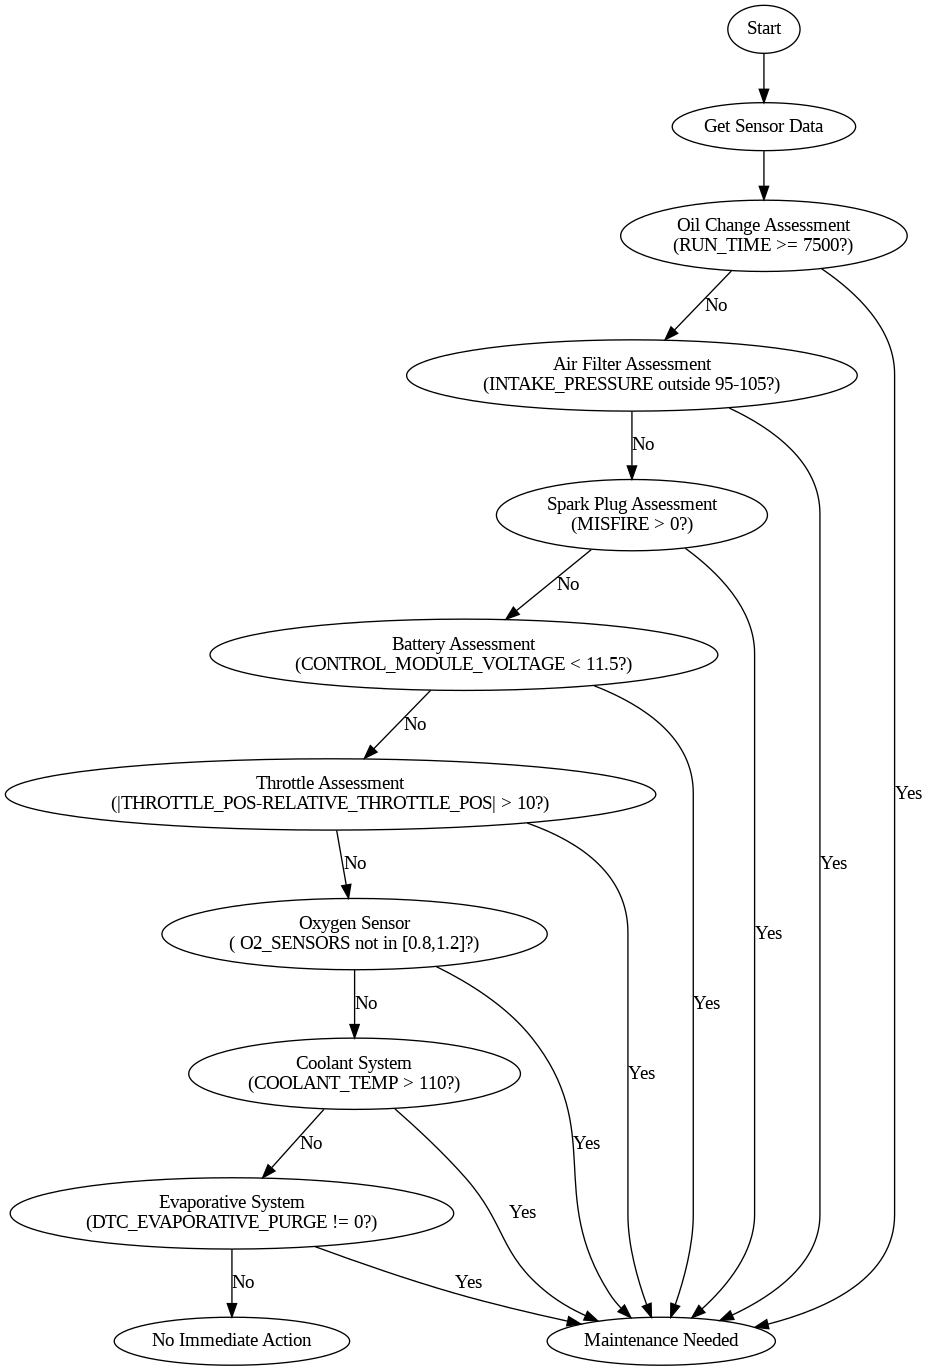
\includegraphics[width=0.9\textwidth]{assets/predictive-maintainance.png}
            \caption{Comprehensive Flowchart of the Predictive Maintenance Router Diagnostic Process}
            \label{fig:predictive-maintenance-flowchart}
        \end{figure}
    \end{enumerate}

\section{MOBILE APPLICATION}
    The ADAM system’s mobile application serves as the primary user interface for data visualization and user interaction. Built using cross-platform frameworks like React Native or Flutter, the app is designed for both Android and iOS devices, ensuring wide accessibility.
    \begin{itemize}
        \item \textbf{Real-Time Monitoring:} The app provides real-time updates on vehicle diagnostics, including engine health, fuel efficiency, and emission compliance. Users can view live data streams from the OBD-II interface, allowing them to monitor their vehicle's performance on-the-go.
        \item \textbf{Maintenance Alerts:} Users receive notifications for upcoming maintenance tasks based on predictive analytics. The app alerts users about required services such as oil changes, tire rotations, and brake inspections, helping them stay proactive in vehicle care.
        \item \textbf{Driver Behavior Analytics:} The app tracks driver behavior metrics such as acceleration patterns, braking habits, and speed compliance. This data is visualized through intuitive graphs and charts, enabling users to improve their driving habits for better fuel efficiency and safety.
        \item \textbf{Emission Compliance Status:} Users can check their vehicle's emission status against regulatory standards. The app provides insights into emission levels and compliance with local environmental regulations.
        \item \textbf{User-Friendly Interface:} The mobile app features a clean and intuitive design that allows users to easily navigate through various sections, access detailed reports, and interact with the system without technical expertise.
        \item \textbf{Chatbot Integration:} The app includes a chatbot that allows users to ask questions about their vehicle's performance, maintenance schedules, and diagnostic results. The chatbot provides instant responses, making it easy for users to get information without navigating through complex menus.
    \end{itemize}
    The mobile application serves as the primary interface for users to interact with the ADAM system, providing a seamless experience for monitoring vehicle performance, receiving maintenance alerts, and accessing diagnostic information

    \begin{figure}[h]  % 'h' means place here
    \centering
    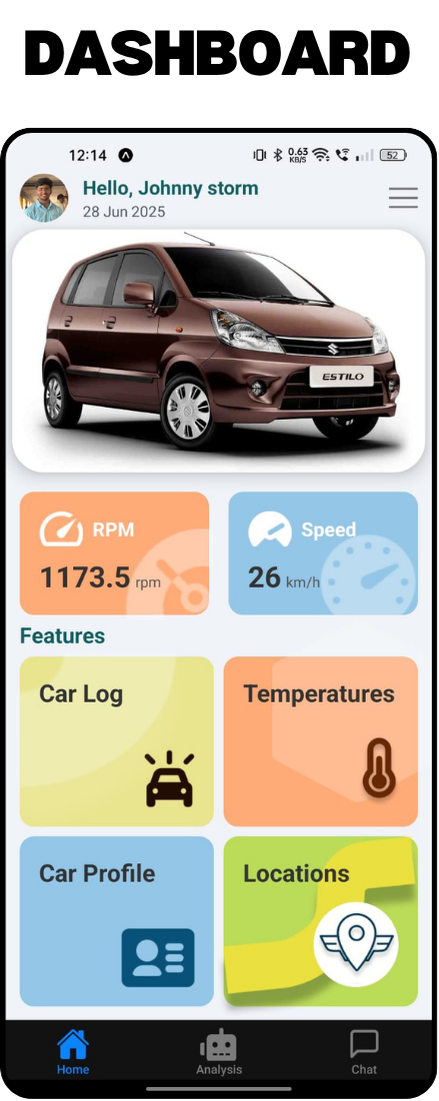
\includegraphics[width=0.2\textwidth]{assets/Dashboard.png}
    \caption{Dashboard of the ADAM mobile application}
    \label{fig:ADAM Box}
    \end{figure}

    \begin{figure}[h]  % 'h' means place here
    \centering
    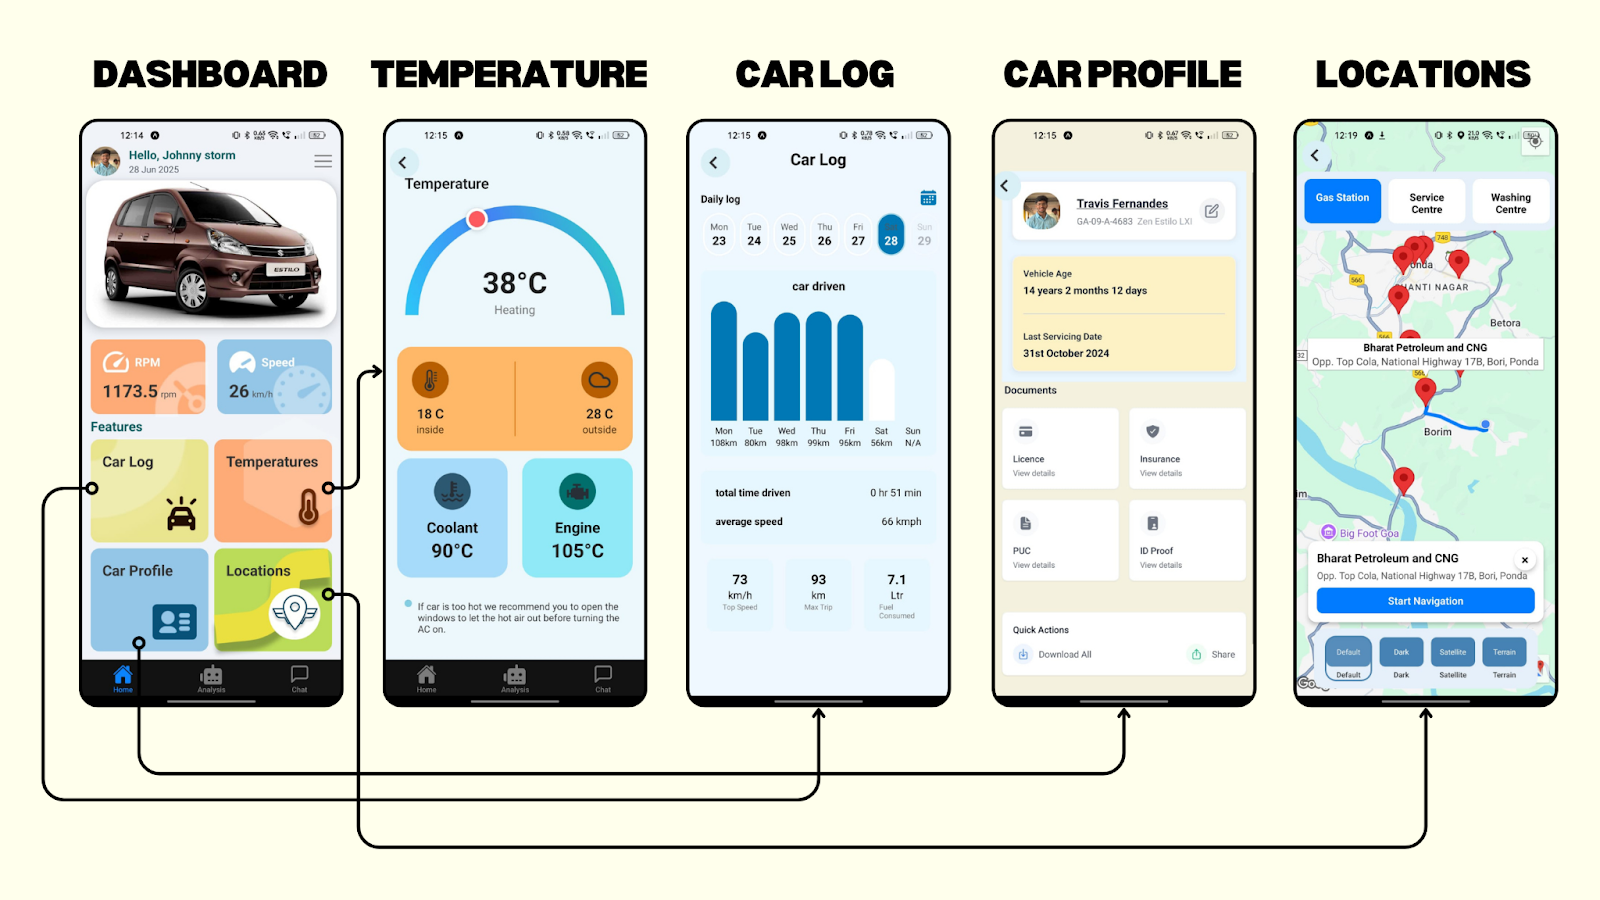
\includegraphics[width=1\textwidth]{assets/Dashboard-Arrows.png}
    \caption{The dashboard includes direct navigation to four essential modules}
    \label{fig:ADAM Box}
    \end{figure}

    \begin{figure}[h]  % 'h' means place here
    \centering
    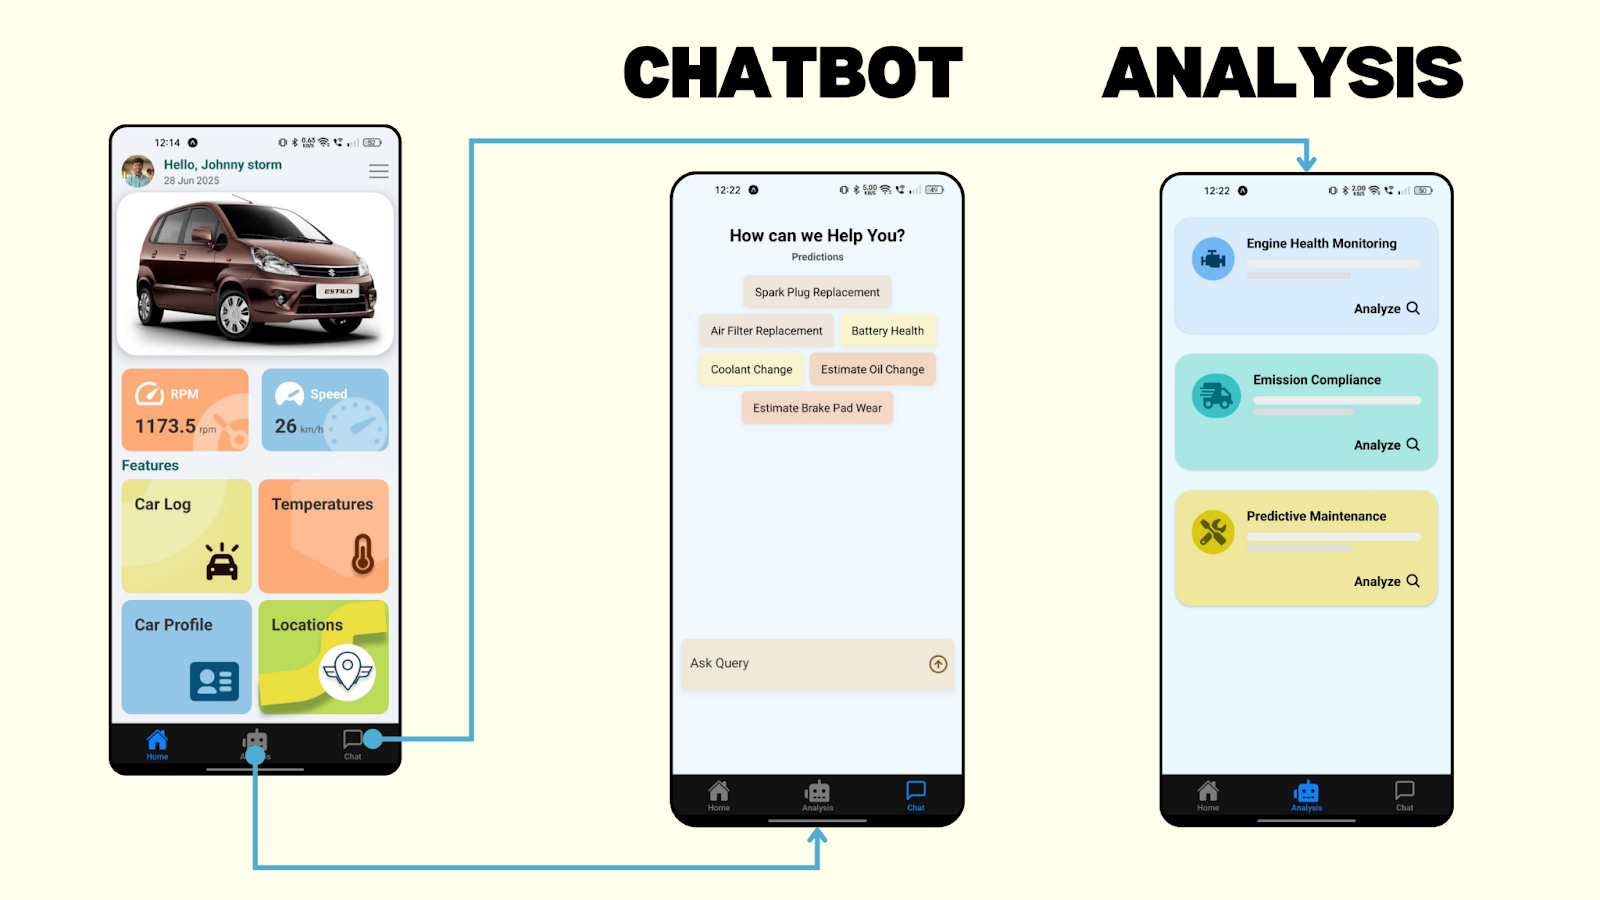
\includegraphics[width=1\textwidth]{assets/App-Bottom-Tab.png}
    \caption{The bottom tab of the ADAM mobile application provides quick access to key features}
    \label{fig:ADAM Box}
    \end{figure}
